\documentclass[11pt]{article}

% ---------- Preamble ----------
\usepackage[a4paper,margin=1in]{geometry}
\usepackage{amsmath}
\usepackage{mathptmx}
\usepackage[scaled=0.92]{helvet}
\usepackage{microtype}
\usepackage[dvipsnames]{xcolor}
\usepackage{tikz}
\usetikzlibrary{positioning,fit,backgrounds,arrows.meta,calc,shapes.geometric}
\usepackage{booktabs}
\usepackage{array}
\usepackage{enumitem}
\usepackage[hidelinks]{hyperref}
\usepackage{caption}
\captionsetup{font=small,labelfont=bf}

\definecolor{caindigo}{HTML}{4F46E5}
\definecolor{cagreen}{HTML}{059669}
\definecolor{caorange}{HTML}{EA580C}
\definecolor{caslate}{HTML}{475569}
\definecolor{cared}{HTML}{DC2626}
\definecolor{caviolet}{HTML}{8B5CF6}
\definecolor{cabgindigo}{HTML}{EEF2FF}
\definecolor{cabggreen}{HTML}{ECFDF5}
\definecolor{cabgorange}{HTML}{FFF7ED}
\definecolor{cabgslate}{HTML}{F8FAFC}
\definecolor{cabgred}{HTML}{FEF2F2}
\definecolor{cabgviolet}{HTML}{F5F3FF}

\newcommand{\invariant}[1]{\textbf{I#1}}
\newcommand{\rulename}[1]{\texttt{#1}}

\title{\textbf{CrossAudit: A Git-Native, Cross-Vendor Audit Loop\\for Agentic Science}}
\author{Zhaohe Dong\\[2pt]
\normalsize Independent Researcher\\
\normalsize \texttt{dongzhaohe321418@gmail.com}}
\date{July 2026}

\begin{document}
\maketitle

\begin{abstract}
\noindent Autonomous ``AI scientist'' systems increasingly generate, execute, and review research. In current frontier systems, however, the reviewing agent is an internal critic chosen by the same operator --- often from the same model family or vendor as the generating agent --- exposing supervision to self-preference bias and to blind spots shared across a common training pipeline; the supervision trace, moreover, usually lives in opaque platform logs rather than in an artefact a third party can replay. We present \textbf{CrossAudit}, a lightweight, infrastructure-minimal protocol for supervising autonomous research pipelines, built on three commitments: (i)~\emph{heterogeneity} --- every experiment increment produced by a generator agent is audited by an agent from a different model vendor, against a versioned, human-authored rulebook (the \emph{Constitution}); (ii)~a \emph{git-native ledger} --- experiments, audit reports, verdicts, disputes and escalations are all commits, so the entire supervision history is replayable, diffable and citable; and (iii)~\emph{graded, escalation-based human oversight} --- deterministic, model-free checks and hard inconsistencies gate the pipeline, judgement calls do not, and a bounded revision loop escalates unresolved blockers to a human principal. We specify the protocol as six invariants, describe a reference implementation built entirely from GitHub Actions and a few hundred lines of dependency-light Python, and report a live deployment of a closely related variant in a computational-chemistry pipeline whose generator (Claude-based), auditor (GPT-lineage), and compute (cloud HPC) are mutually decoupled. We argue that cross-vendor audit trails of this kind offer a practical, immediately adoptable substrate for accountable machine science.
\end{abstract}

% ---------- 1 Introduction ----------
\section{Introduction}\label{sec:intro}

Two developments frame this paper. The first is the arrival of genuinely agentic research systems: pipelines in which large language model (LLM) agents propose hypotheses, write and execute code, run experiments, and draft manuscripts with limited human intervention. Sakana's AI Scientist produced machine-generated papers end-to-end \cite{lu2024aiscientist,yamada2025aisv2} and has since seen machine-led work reach peer-reviewed venues \cite{lu2026nature}; DeepMind's AI co-scientist organises hypothesis generation as a multi-agent tournament \cite{gottweis2025coscientist}; autonomous laboratories close the loop through to physical synthesis \cite{boiko2023,szymanski2023}. Publishers and funders are already being urged to respond institutionally \cite{naturenews2026}.

The second development is older and less glamorous: science's continuing struggle with reliability. A majority of surveyed researchers have failed to reproduce a published result \cite{baker2016}. Agentic pipelines raise the stakes on both sides of this ledger. They can enforce discipline no human sustains --- every increment logged, every parameter recorded --- or they can mass-produce plausible, well-formatted, wrong results faster than any human audit culture can absorb.

The critical question is therefore not whether machine-generated science should be supervised, but \emph{by what mechanism}, and \emph{by whom}. Current frontier systems embed supervision \emph{inside} the system: a reflection agent, an automated reviewer, a ranking tournament \cite{lu2024aiscientist,gottweis2025coscientist}. These internal critics share a structural weakness: critic and creator are instantiated from the same model or, at best, the same vendor's training pipeline. LLM evaluators are known to systematically favour outputs resembling their own generations --- self-preference bias, with self-recognition capability causally implicated \cite{panickssery2024}; judge-position and style biases compound the problem \cite{zheng2023}. Two agents that share a training distribution share blind spots, and a reviewer that shares the author's blind spots approves precisely the author's characteristic errors. Meanwhile, the supervision trace of most agentic systems --- who flagged what, what was revised, what was waved through --- lives in ephemeral context windows or proprietary platform logs, invisible to the communities that will be asked to trust the resulting science.

\paragraph{Contributions.} This paper makes four contributions.
\begin{enumerate}[itemsep=1pt,topsep=3pt]
  \item We articulate the \emph{same-source supervision problem} in agentic science: internal critique by same-vendor models is structurally exposed to correlated failure (\S\ref{sec:related}).
  \item We specify \textbf{CrossAudit}, a supervision protocol defined by six invariants --- vendor heterogeneity, ledger completeness, citation validity, determinism-first, bounded revision, and graded interruption --- that together yield a replayable, third-party-auditable supervision history (\S\ref{sec:protocol}).
  \item We describe a reference implementation requiring no infrastructure beyond two git repositories, a CI service, and two model API keys, together with a live deployment of a closely related variant in the author's computational-chemistry pipeline (\S\ref{sec:implementation}).
  \item We give an explicit threat model, including the attacks the protocol does \emph{not} withstand, and situate the design against plausible alternatives (\S\ref{sec:threat}--\S\ref{sec:discussion}).
\end{enumerate}

CrossAudit is deliberately modest in its claims. It does not certify scientific truth; no textual audit can. It certifies something narrower and checkable: that every increment of a machine-generated research record passed, or failed, a named set of versioned rules, applied by an agent with no stake in the increment's acceptance, with the whole exchange preserved verbatim in the ledger, public wherever the operator publishes it. We contend that this narrower property is the right first target for accountable machine science, plausibly for the same reason continuous integration --- not formal verification --- became the load-bearing quality mechanism of modern software.

% ---------- 2 Related work ----------
\section{Related work and the same-source problem}\label{sec:related}

\paragraph{Agentic science systems.} The AI Scientist \cite{lu2024aiscientist,yamada2025aisv2,lu2026nature} automates the ideation--experiment--writeup--review cycle, including an internal automated reviewer scored against human reviewer data. The AI co-scientist \cite{gottweis2025coscientist} structures generation--reflection--ranking--evolution agents into a self-improving tournament over hypotheses, with reported expert-validated outcomes in drug repurposing and antimicrobial resistance. Language agents for literature synthesis reach or exceed expert performance on retrieval-grounded tasks \cite{skarlinski2024}. In the laboratory, Coscientist executed chemistry protocols from natural-language goals \cite{boiko2023} and A-Lab ran autonomous materials synthesis campaigns \cite{szymanski2023}. Across all of these, quality control is architecturally \emph{internal}: reviewer agents, reflection stages, or tournament judges chosen and hosted by the same operator, inside the same platform, with no commitment to vendor heterogeneity --- and frequently instantiated from the same model family as the generators they judge.

\paragraph{Why internal critique is not enough.} Panickssery et al.\ demonstrate that LLM evaluators recognise their own generations and rate them preferentially, with fine-tuning experiments showing self-recognition capability \emph{causes} the inflation \cite{panickssery2024}. Zheng et al.\ catalogue further judge pathologies --- position, verbosity, and self-enhancement biases --- even in strong models \cite{zheng2023}. These results concern single-model self-evaluation; we hypothesise the mechanism generalises: models sharing a training pipeline are likely to share stylistic priors and knowledge gaps, putting a same-vendor critic at the wrong end of the bias distribution precisely when it matters. We call this the \emph{same-source supervision problem}. Cross-vendor pairing does not eliminate correlated error --- all frontier models ingest substantially the same public literature, so where the literature is wrong, both can be confidently wrong together --- but it removes the best-documented bias in this setting (self-preference) and is intended to decorrelate vendor-idiosyncratic failure modes. What cross-vendor pairing cannot fix, a model-free layer must (\S\ref{sec:protocol}, \invariant{4}).

\paragraph{Supervision as an artefact.} Software engineering solved an analogous trust problem not by making programmers infallible but by making quality mechanisms \emph{inspectable}: version control, continuous integration, review trails. Reproducibility initiatives in science point the same way --- the unit of trust is the auditable record, not the author's competence \cite{baker2016}. CrossAudit transplants this stance to agentic science: the supervision history itself becomes a first-class, versioned, citable research artefact.

% ---------- 3 Protocol ----------
\section{The CrossAudit protocol}\label{sec:protocol}

\subsection{Objects and roles}\label{sec:roles}

CrossAudit supervises a pipeline in which a \textbf{Generator} agent (vendor $A$) produces discrete \emph{experiment increments} --- commits under a designated path of a \textbf{Science Repository}. Each increment is audited by an \textbf{Auditor} agent (vendor $B \neq A$) against a versioned, human-authored rulebook, the \textbf{Constitution}, held with all \emph{audit reports} in a separate \textbf{Audit Repository}. A \textbf{Deterministic Check Layer} (DCL) --- plain scripts with no learned component: schema validation, unit and dimension analysis, convergence assertions, provenance completeness --- runs before any model reads anything. A \textbf{Human Principal} authors the Constitution and receives escalations, but sits deliberately outside the per-increment loop. Compute (in the reference deployment, jobs on cloud HPC) is decoupled from supervision: verdicts gate the \emph{next} increment, never running jobs.

The two-repository split is separation of powers made mechanical: the Auditor holds no write access to the Science Repository, the Generator none to the Audit Repository, so neither agent holds credentials to alter the other's record; guarding each record against its \emph{own} author additionally requires branch protection.

\begin{figure}[t]
\centering
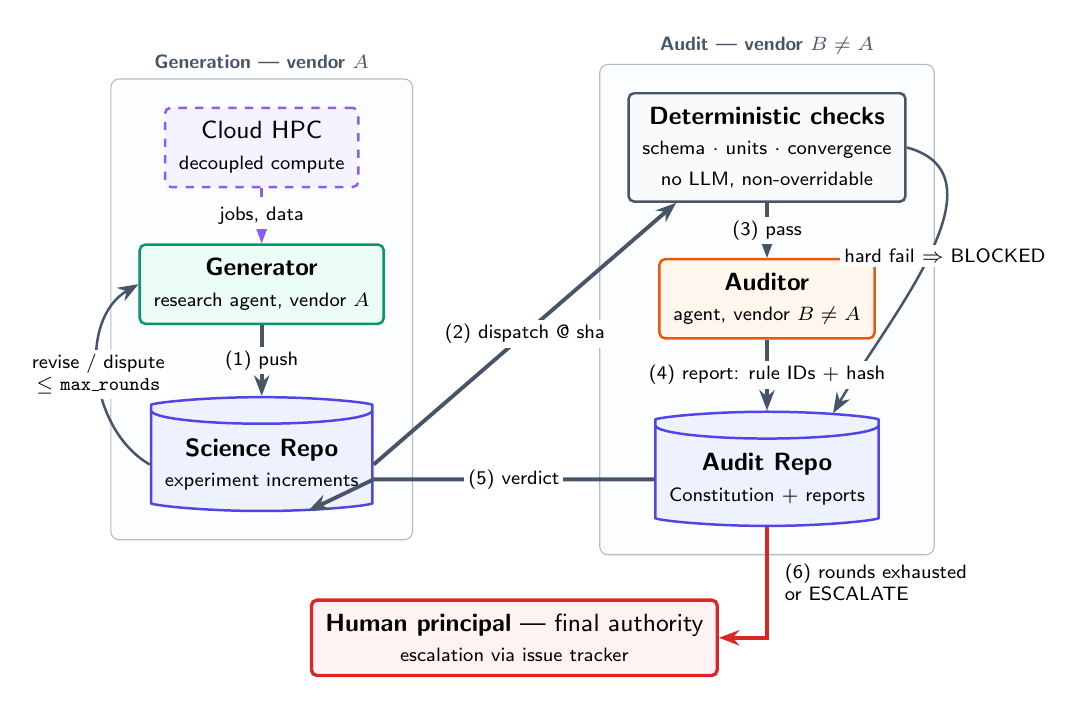
\begin{tikzpicture}[
  font=\small\sffamily,
  node distance=7mm and 12mm,
  box/.style={draw, rounded corners=2pt, align=center, inner sep=5pt, minimum height=9mm, line width=0.9pt},
  repo/.style={box, cylinder, shape border rotate=90, aspect=0.12, draw=caindigo, fill=cabgindigo},
  gen/.style={box, draw=cagreen, fill=cabggreen},
  aud/.style={box, draw=caorange, fill=cabgorange},
  det/.style={box, draw=caslate, fill=cabgslate},
  hum/.style={box, draw=cared, fill=cabgred, line width=1.2pt},
  hpc/.style={box, draw=caviolet, fill=cabgviolet, dashed},
  flow/.style={-{Stealth[length=2.6mm]}, line width=0.9pt, draw=caslate},
  main/.style={flow, line width=1.4pt},
  lbl/.style={fill=white, inner sep=1.5pt, font=\scriptsize\sffamily}
]
% Left lane: generation
\node[hpc] (hpc) {Cloud HPC\\ \scriptsize decoupled compute};
\node[gen, below=of hpc] (gen) {\textbf{Generator}\\ \scriptsize research agent, vendor $A$};
\node[repo, below=9mm of gen] (sci) {\textbf{Science Repo}\\ \scriptsize experiment increments};
% Right lane: audit
\node[det, right=34mm of hpc] (dcl) {\textbf{Deterministic checks}\\ \scriptsize schema $\cdot$ units $\cdot$ convergence\\ \scriptsize no LLM, non-overridable};
\node[aud, below=of dcl] (audr) {\textbf{Auditor}\\ \scriptsize agent, vendor $B \neq A$};
\node[repo, below=9mm of audr] (arepo) {\textbf{Audit Repo}\\ \scriptsize Constitution $+$ reports};
% Human
\node[hum, below=10mm of $(sci.south)!0.5!(arepo.south)$] (human) {\textbf{Human principal} --- final authority\\ \scriptsize escalation via issue tracker};
% Edges
\draw[flow, dashed, draw=caviolet] (hpc) -- node[lbl]{jobs, data} (gen);
\draw[main] (gen) -- node[lbl]{(1) push} (sci);
\draw[main] (sci.east) -- node[lbl]{(2) dispatch @ sha} ($(dcl.south west)!0.35!(dcl.south)$);
\draw[main] (dcl) -- node[lbl]{(3) pass} (audr);
\draw[flow] (dcl.east) to[out=-15,in=60] node[lbl, xshift=2mm]{hard fail $\Rightarrow$ BLOCKED} (arepo.north east);
\draw[main] (audr) -- node[lbl]{(4) report: rule IDs $+$ hash} (arepo);
\draw[main] (arepo.west) -- node[lbl]{(5) verdict} (sci.east |- arepo.west) -- (sci.south east);
\draw[flow] (sci.west) to[out=150,in=210] node[lbl, align=center]{revise / dispute\\ $\leq$ \texttt{max\_rounds}} (gen.west);
\draw[main, draw=cared] (arepo.south) |- node[lbl, pos=0.25, right=1.5mm, align=left]{(6) rounds exhausted\\ or ESCALATE} (human.east);
% Lane frames
\begin{scope}[on background layer]
  \node[draw=caslate!40, rounded corners=3pt, fill=cabgslate!40, fit=(hpc)(gen)(sci), inner sep=3.5mm, label={[font=\scriptsize\sffamily\bfseries, text=caslate]north:Generation --- vendor $A$}] {};
  \node[draw=caslate!40, rounded corners=3pt, fill=cabgslate!40, fit=(dcl)(audr)(arepo), inner sep=3.5mm, label={[font=\scriptsize\sffamily\bfseries, text=caslate]north:Audit --- vendor $B \neq A$}] {};
\end{scope}
\end{tikzpicture}
\caption{The CrossAudit loop. Solid numbered arrows follow one experiment increment; the deterministic layer runs before any model (\invariant{4}); the revision loop is bounded (\invariant{5}); humans are interrupted only by escalation (\invariant{6}).}
\label{fig:arch}
\end{figure}

\subsection{Six invariants}\label{sec:invariants}

An implementation is CrossAudit exactly when it preserves the following.

\begin{description}[itemsep=2pt,topsep=3pt]
  \item[\invariant{1} --- Heterogeneity.] The Auditor's model family differs from the Generator's. This removes the demonstrated self-evaluation channel of self-preference bias by construction \cite{panickssery2024}, and is designed to decorrelate vendor-idiosyncratic failure modes --- an effect this paper does not measure (\S\ref{sec:implementation}).
  \item[\invariant{2} --- Ledger completeness.] Every protocol artefact --- increment, report, verdict, dispute, escalation, and every change to the Constitution --- is a commit (or an issue) in one of the two repositories. No supervision state lives only in model context or platform logs. The history is replayable by a third party from the repositories alone --- replay of the \emph{record}; the model calls behind it are stochastic and not re-executable.
  \item[\invariant{3} --- Citation validity.] An audit report must cite the rule IDs it applied and the commit hash of the Constitution version in force. A report that cites nothing, or an unverifiable version, is \emph{invalid} and treated as an Auditor failure --- it escalates; it can never pass an increment.
  \item[\invariant{4} --- Determinism first.] The DCL runs before any LLM audit. A DCL hard failure yields \texttt{BLOCKED} regardless of any model's opinion, and no model may waive a DCL verdict. Rationale: heterogeneous models still share the public corpus and hence its errors; the supervision layer whose failure modes are least entangled with any model is one with no learned component at all.
  \item[\invariant{5} --- Bounded revision.] At most \texttt{max\_rounds} Generator--Auditor exchanges per increment (default three). Exhaustion escalates. This is the oscillation guard: without it, two mutually-correcting agents can disagree indefinitely, each round locally plausible and the pair jointly divergent.
  \item[\invariant{6} --- Graded interruption.] Findings carry exactly two severities. \texttt{BLOCKER} (objective defect: DCL failure, internal contradiction, missing provenance, method--declaration mismatch) gates the increment. \texttt{ADVISORY} (judgement: parameter taste, style, scope) is recorded for asynchronous human reading and never gates. Humans are interrupted only by \texttt{ESCALATE}. Running compute is never interrupted at all.
\end{description}

Two severities, deliberately. In our judgement every additional level invites severity-inflation negotiation between the agents; where a finer distinction is needed it belongs in the rule's acceptance criterion, not in the escalation lattice.

\subsection{The Constitution}\label{sec:constitution}

The Constitution is the protocol's quality ceiling: the Auditor's blocking power cannot exceed the rules it is given, and the Generator is free to exploit whatever the rules fail to say. CrossAudit therefore treats it as law rather than documentation. Every rule carries a stable identifier (\rulename{CA-DATA-001}), a severity, a path scope, a \emph{decidable} acceptance criterion, and a rationale. Decidability is the load-bearing requirement: a criterion a competent reader can evaluate against named artefacts without further judgement. What cannot be phrased decidably is either demoted to \texttt{ADVISORY} or --- better --- mechanised and moved into the DCL. Meta-rules govern the audit itself: missing evidence is a finding, never an implicit pass (\rulename{CA-META-001}); a report without citations is invalid (\rulename{CA-META-002}, enforcing \invariant{3}); the Auditor may not issue a \texttt{BLOCKER} without citing a \texttt{BLOCKER}-severity rule --- it does not legislate taste (\rulename{CA-META-003}); and matters beyond the increment-plus-Constitution evidence base must escalate rather than be guessed (\rulename{CA-META-004}). Constitution changes are commits reviewed by the human principal; the loop can propose rules but never enact them.

\subsection{Rounds, disputes, termination}\label{sec:rounds}

Round $k$ for an increment: the Auditor publishes report $R_k$ with a verdict. On \texttt{BLOCKED}, the Generator either \emph{revises} (a new commit, opening round $k{+}1$) or \emph{disputes} specific findings by rule ID, with grounds. A disputed finding returns to the Auditor once: it is withdrawn with a logged reason, or upheld. An upheld dispute at the round bound escalates. Disputes exist because the Auditor is fallible in both directions --- a false-positive \texttt{BLOCKER}, silently obeyed, degrades the science as surely as a false negative --- and the one-shot rule prevents the dispute channel from becoming the oscillation it exists to control. Termination is structural: each increment ends in \texttt{PASS} or in human hands after at most \texttt{max\_rounds} exchanges.

% ---------- 4 Implementation ----------
\section{Reference implementation and deployment}\label{sec:implementation}

\subsection{Mechanics}

The reference implementation\footnote{\url{https://github.com/dongzhaohe321418-lab/crossaudit} (MIT licence).} uses no infrastructure beyond GitHub itself. A push under \texttt{experiments/} triggers a cross-repository dispatch carrying the commit SHA, changed paths, and round number (read from a commit trailer). The Audit Repository's workflow checks out the science repository \emph{pinned at the audited SHA}, asserts \invariant{1} from configuration, runs the DCL, then invokes the Auditor via an OpenAI-compatible endpoint with the Constitution, the DCL output, and the increment content as fenced data. The report is committed to the ledger; the verdict is dispatched back; the science repository routes it --- proceed, revise, or open an escalation issue. The whole implementation is three workflow files and two Python programs (a check runner and an auditor runner) of a few hundred dependency-light lines; configuration is a single \texttt{crossaudit.yml} declaring vendors, \texttt{max\_rounds}, and escalation policy.

Three implementation details carry protocol weight. First, the auditor runner validates the model's reply against a fixed schema --- verdict, findings with severities and rule citations --- and any malformed or citation-free reply is converted to \texttt{ESCALATE} (\invariant{3}); a common failure shape of an LLM judge --- the confident empty report --- is thereby converted from silent passage into an escalation. Second, increment content is passed to the Auditor as fenced, size-bounded content with the system prompt instructing that embedded instructions be ignored --- a best-effort defence whose residual risk \S\ref{sec:threat} states plainly; the reference Auditor has no tools. Third, verdict synthesis is code, not model output: DCL hard failures dominate any model verdict (\invariant{4}).

\subsection{A live deployment}

CrossAudit runs live in the author's computational-chemistry pipeline (perovskite additive screening). The generation side is a Claude-based research agent that plans calculations, launches them on Alibaba Cloud E-HPC and a GPU worker, and pushes every increment to a private science repository whose audit policy --- an epistemic-status ledger separating established, bounded, and provisional claims, together with a standing retraction log --- is itself a committed, versioned document. The audit side is orchestrated by a controller that opens a \emph{cycle} against a fixed science commit: the audit request pins a SHA-256 evidence manifest covering every tracked file, and a Codex-CLI auditor (OpenAI lineage, so \invariant{1} holds against the Claude-based generator) writes exactly four artifacts into an append-only per-cycle directory of a separate audit repository --- human-readable report, machine-readable result, run metadata, and a per-file hash manifest --- on a single long-lived \texttt{audit} branch that later cycles are forbidden to rewrite, the prohibition enforced by controller validation of every audit commit before a cycle is recorded as final. The controller's own orchestration state deliberately lives outside both repositories, so tampering by either agent with the record of its own supervision is detectable against controller-held state. Two deliberate divergences from the reference design should be named plainly: the deployed auditor is a tool-bearing CLI agent rather than the reference's toolless one, contained instead by that commit validation and the append-only cycle layout; and the externalised controller state means the deployment's history is fully replayable from the repositories \emph{plus} that state --- a weaker property than \invariant{2}'s repositories-alone ideal. Every input and output lives on GitHub; the system is designed so that any single component --- generator, auditor, controller host, workstation --- can fail without loss of ledger state.

Two refinements of the deployed system go beyond the reference implementation and are worth adopting upstream. First, findings are \emph{evidence-typed}: each carries a policy citation (section and rule ID), a deterministic check identifier where applicable, and a copy-paste \emph{reproduce} command, so a human can re-derive any deterministic finding in seconds. Second, blocking is \emph{scope-granular}: a finding blocks named scopes --- production-job submission, claim publication --- rather than the pipeline wholesale, refining \invariant{6}'s graded-interruption principle. Human authority appears as the protocol's escalation-only interruption plus one deployment-specific addition: a standing principal-approval gate on production launches, recorded in the ledger. The loop is live in the plainest sense: at the time of writing, its most recent cycle --- opened and closed within six minutes on the morning of writing --- returned a \texttt{BLOCK} decision on deterministic grounds (manifest-hash disagreements and commit-provenance defects), freezing production submission and claim publication until resolved. Audits gate the research record, not the queue; running E-HPC jobs are never interrupted.

Costs are modest by construction. The DCL is free. LLM audit cost scales with the size of the \emph{increment}, not of the computation behind it: auditing a few hundred lines of results and metadata costs cents, while the experiment it certifies may represent hours of HPC time. Supervision priced at the documentation it reads rather than the compute it certifies is an unusually cheap layer of assurance --- with the caveats that multi-round exchanges multiply audit calls, and that escalations spend human time, the system's true scarce resource.

We deliberately make no quantitative claims about detection rates here. The honest evaluation --- seeded-defect recall across heterogeneous versus homogeneous auditor pairings, false-positive burden, escalation precision --- requires a defect corpus and is future work (\S\ref{sec:threat}); the present paper's claim is architectural, and the deployment's role is existence proof for the deployed variant: the loop runs unattended, at single-researcher scale, on commodity infrastructure. The one concrete catch reported above is attributable to the deterministic layer; this paper claims no LLM-layer catches.

% ---------- 5 Threat model ----------
\section{Threat model and limitations}\label{sec:threat}

We state plainly what CrossAudit withstands and what it does not.

\begin{itemize}[itemsep=2pt,topsep=3pt]
  \item \textbf{Self-preference and vendor-correlated error} are addressed by \invariant{1}. \emph{Corpus}-correlated error is not: where the shared literature is wrong or outdated, both vendors can agree confidently and wrongly. Mitigation is \invariant{4} for everything mechanisable, and the human's asynchronous reading of \texttt{ADVISORY} trails for what is not. This residual cannot be assumed reducible by adding more LLM auditors, since all ingest substantially the same public literature.
  \item \textbf{Prompt injection.} An increment could embed text addressing the Auditor. The Auditor runs toolless against a fixed reply schema with content fenced as data; and because DCL verdicts are non-overridable, injection cannot waive the layer where hard defects are caught. Injection shaping the \emph{LLM-side} report remains partially open, as it does for all current LLM-judge systems \cite{zheng2023}.
  \item \textbf{Auditor failure} --- empty, malformed, or rule-free reports --- converts to escalation (\invariant{3}), never to silent passage. The cost is human attention, which is the correct currency for an unreliable auditor.
  \item \textbf{Oscillation and deadlock} are bounded by \invariant{5}; the failure mode degrades to a human decision with the full exchange on the ledger, which is the intended floor.
  \item \textbf{Goodharting the Constitution.} A capable Generator will satisfy the letter of decidable rules. Decidability makes this visible rather than solved: the human reviews rule--outcome drift on the ledger and legislates accordingly. The Constitution is a living document; its growth from escalations is the system learning.
  \item \textbf{Collusion} has no covert channel --- the agents share no channel except committed artefacts, so any coordination must occur in public, on the record, where it is at least inspectable. Convergent style over many rounds is the realistic soft risk, met by Constitution review cadence.
  \item \textbf{Vendor identity is self-declared.} The ledger proves an exchange occurred, not the identity of the models behind OpenAI-compatible endpoints; \invariant{1} is asserted from configuration, not verified cryptographically. Attested inference or vendor-signed responses would close this; today it is an honest limit on what ``third-party-auditable'' can mean.
  \item \textbf{Confidentiality.} The protocol ships every increment --- possibly unpublished, patentable material --- to a second vendor's API. Data governance of that call (agreements, retention, disclosure risk) sits outside the protocol and must be settled per deployment.
  \item \textbf{Scope.} CrossAudit audits the research \emph{record}, not the world: it cannot detect a miscalibrated instrument, a wrong dataset honestly described, or fraud upstream of the repository. It is also currently specified for single-generator pipelines; multi-agent generation raises attribution questions we do not address here.
\end{itemize}

% ---------- 6 Discussion ----------
\section{Discussion}\label{sec:discussion}

\paragraph{Continuous integration for scientific claims.} The precise ambition of CrossAudit is the one CI achieved for software: not proof of correctness, but a cheap, always-on, inspectable floor under quality, with human judgement redeployed to where it discriminates --- the rules, the escalations, and the science --- rather than spent uniformly on every increment. The analogy holds, we believe, in one further respect: CI spread without institutional permission --- a single developer could adopt it unilaterally, and its artefacts (badges, logs) became social proof. One disanalogy must be owned: CI's checks are deterministic while CrossAudit's distinctive layer is a stochastic judge; the DCL exists precisely to keep the gate's hard core deterministic. CrossAudit is designed for the same adoption path: one researcher, two repositories, an afternoon.

\paragraph{Relation to platform-scale systems.} CrossAudit is complementary to, not competitive with, systems such as the AI co-scientist \cite{gottweis2025coscientist} or the AI Scientist \cite{lu2026nature}. Those systems generate; CrossAudit supervises whatever generates. Indeed the sharpest version of our proposal is addressed to exactly such platforms: internal critique stages are architecturally straightforward to re-instantiate across vendor lines and to externalise onto public ledgers (the organisational and confidentiality costs are not ours to estimate), and the resulting audit trails would give publishers and funders --- currently being asked to trust process descriptions \cite{naturenews2026} --- something they can actually inspect.

\paragraph{What the ledger buys science socially.} A complete supervision history, public where the operator publishes it, changes the character of machine-generated results. A claim arrives not as prose plus reputation but as prose plus its audit record: which rules it was checked against, what was contested, what a differently-trained model conceded or refused. Reviewers can spot-check the ledger instead of re-deriving trust from nothing. Failed audits are data too: a public record of what auto-generated science gets wrong, per rule and per field, is precisely what the community lacks in the current platform era.

\paragraph{The ledger as a data asset.} A CrossAudit deployment produces, as a by-product, something the field currently largely lacks: a corpus of \emph{supervised machine science}. Each (increment, findings, dispute, resolution) tuple is a labelled example of scientific work judged by an independent party under explicit rules --- high-grade training signal for better generator and auditor agents alike. Aggregated across deployments, failed audits form a public error taxonomy of agentic research: what machine-generated science actually gets wrong, per rule, per field, over time. Whoever runs the loop accumulates this asset; a community that runs it openly accumulates it as a commons.

\paragraph{Constitutions as community objects.} Because the Constitution is a plain, forkable file with stable rule IDs, it can outgrow any single deployment: a research community can maintain a shared domain constitution the way communities maintain style guides and lint rules; a journal could publish the constitution it expects machine-assisted submissions to have been audited under, and accept the ledger link alongside the manuscript, exactly as data-availability statements are accepted today; funders could write ``public supervision ledger'' into terms. For regulated settings (pharmaceutical and clinical computation among them), the ledger's attributability and contemporaneous, hash-manifested record resemble properties audit regimes already demand of human work, though we claim compliance with no specific regime. And a repository badge --- increments audited, escalations raised, constitution version --- would do for machine science what CI badges did for software: compress an inspectable process into a glanceable, verifiable signal. None of this requires new technical infrastructure; it requires only that the artefact exist, which a conforming deployment produces.

\paragraph{Management by exception, at research scale.} As agent labour becomes cheap, the binding constraint of agentic science shifts from compute to human attention. CrossAudit's economic content is a reduction in \emph{gating} cost from $O(\text{increments})$ to $O(\text{escalations})$ --- conditional on escalation volume staying low, which the author observes informally but has not measured --- with advisory reading batched or sampled rather than per-increment. This is the managerial precondition for one researcher credibly directing several agent pipelines at once --- and it should in principle extend beyond science to agentic work products that arrive as discrete increments whose quality is partially rule-expressible, from code to quantitative analysis --- a conjecture this paper does not test.

\section{Conclusion}\label{sec:conclusion}

CrossAudit reframes supervision of autonomous research from a platform feature into a public, versioned artefact produced by structurally independent reviewers. Its ingredients are deliberately unglamorous --- a second vendor, a rulebook with IDs, scripts before models, a bounded loop, and git underneath everything --- because unglamorous ingredients are what individual researchers can adopt today without permission. The protocol's six invariants are a deliberately small set that jointly buys structurally independent review, a re-inspectable history, and human authority at the boundary; everything else in this paper is reference detail, and the reference repositories are public. An AI scientist should not grade its own homework. With two repositories and two API keys, it no longer has to.

\paragraph{Acknowledgements.} The CrossAudit reference implementation and the deployment described in \S\ref{sec:implementation} were developed with the assistance of the very class of agentic tools this paper proposes to supervise; the irony is intended.

% ---------- References ----------
\begin{thebibliography}{10}\small

\bibitem{lu2024aiscientist}
C.~Lu, C.~Lu, R.~T. Lange, J.~Foerster, J.~Clune, and D.~Ha.
\newblock The {AI} {Scientist}: Towards fully automated open-ended scientific discovery.
\newblock \emph{arXiv:2408.06292}, 2024.

\bibitem{yamada2025aisv2}
Y.~Yamada, R.~T. Lange, C.~Lu, S.~Hu, C.~Lu, J.~Foerster, J.~Clune, and D.~Ha.
\newblock The {AI} {Scientist}-v2: Workshop-level automated scientific discovery via agentic tree search.
\newblock \emph{arXiv:2504.08066}, 2025.

\bibitem{lu2026nature}
C.~Lu, C.~Lu, R.~T. Lange, Y.~Yamada, S.~Hu, J.~Foerster, D.~Ha, and J.~Clune.
\newblock Towards end-to-end automation of {AI} research.
\newblock \emph{Nature}, 651:914--919, 2026.

\bibitem{gottweis2025coscientist}
J.~Gottweis, W.-H. Weng, A.~Daryin, T.~Tu, et~al.
\newblock Towards an {AI} co-scientist.
\newblock \emph{arXiv:2502.18864}, 2025.

\bibitem{panickssery2024}
A.~Panickssery, S.~R. Bowman, and S.~Feng.
\newblock {LLM} evaluators recognize and favor their own generations.
\newblock In \emph{Advances in Neural Information Processing Systems (NeurIPS)}, 2024.
\newblock arXiv:2404.13076.

\bibitem{zheng2023}
L.~Zheng, W.-L. Chiang, Y.~Sheng, S.~Zhuang, et~al.
\newblock Judging {LLM}-as-a-judge with {MT}-{Bench} and {Chatbot} {Arena}.
\newblock In \emph{Advances in Neural Information Processing Systems (NeurIPS)}, 2023.
\newblock arXiv:2306.05685.

\bibitem{boiko2023}
D.~A. Boiko, R.~MacKnight, B.~Kline, and G.~Gomes.
\newblock Autonomous chemical research with large language models.
\newblock \emph{Nature}, 624:570--578, 2023.

\bibitem{szymanski2023}
N.~J. Szymanski, B.~Rendy, Y.~Fei, R.~E. Kumar, et~al.
\newblock An autonomous laboratory for the accelerated synthesis of novel materials.
\newblock \emph{Nature}, 624:86--91, 2023.

\bibitem{skarlinski2024}
M.~D. Skarlinski, S.~Cox, J.~M. Laurent, J.~D. Braza, et~al.
\newblock Language agents achieve superhuman synthesis of scientific knowledge.
\newblock \emph{arXiv:2409.13740}, 2024.

\bibitem{baker2016}
M.~Baker.
\newblock 1,500 scientists lift the lid on reproducibility.
\newblock \emph{Nature}, 533:452--454, 2016.

\bibitem{naturenews2026}
{Editorial}.
\newblock {AI} scientists are changing research --- institutions, funders and publishers must respond.
\newblock \emph{Nature}, 651:853--854, 2026.

\end{thebibliography}

\end{document}
